\section{Project Overview and Functionality}

The project consists of two main parts:
\begin{itemize}
\item checksumd is the checksum daemon, written in Python. 
\item checksum-monitor is a monitor written in Django that parses log files from checksumd to generate statistics and display details about checksum errors.
\end{itemize}

In addition there is the Lemon integration, but this was purely a configuration task. Please see section \ref{sec:lemon_integration} for details. 

\subsection{Overview of architecture}
An overview of the project can be seen in figure \ref{fig:complete_overview}. The checksumd program runs as a separate application on each disk server. For each file, it computes a checksum, and if there is an error it outputs this to an error log that resides in a folder in AFS. These entries consist of the filename, file size, the checksums, the path returned from the name server, the specifications of the machine (hardware model, hostname, etc.) and more. The same entry is also put in the syslog. 

The checksum-monitor Django application parses the error logs that was stored on AFS. This can be set up as a cron job, or done manually through the web interface. The application will then parse the logs, organize the entries in a relational database, and display it to the clients according to their query preferences.

With regular intervals (e.g. every 24 hours) a summary is also written to the syslog. This summary consists of, among other things, the aggregated numbers for the number of files checked, bad checksums, good checksums, etc. This is then parsed by the Lemon sensor, which is passed to the agent which passes it to the central Lemon database.

\begin{figure}[ht]
\centering
\includegraphics[width=0.7\textwidth]{gfx/complete_overview}
\caption{Architecture overview}
\label{fig:complete_overview}
\end{figure}

\subsection{checksumd}
\label{sec:checksumd_overview}
The checksumd daemon is implemented as a standalone application in Python. In principle, it can be used for other types of machines than CASTOR disk servers as well, but that is not within the scope of this project. This section will give an overview of the daemon.

\subsubsection{Daemon overview}

The process by which the daemon checks files are first by building a queue of all the disks. Each disk has a list of files to be checked (all files under the specified directory, that are not recently modified), and each has an index that points to the next file on the disk. Each of the mount points is assumed to be on a separate disk. At regular intervals, the main thread refreshes the file lists by querying for all files again, and adding new ones and removing deleted ones. 

checksumd is built with threading in mind, and even when only one thread is specified at the command line, a new thread will be spawned to do the actual integrity checking work. The main thread are responsible for housekeeping (e.g. keeping the file list updated and write summaries). This way, housekeeping will not interfer with the actual integrity check operations. 

Until every file on each disk have been checked, each thread will grab one disk, check if it is busy, and if it is not, compute the checksum of the files. If the thread detects that the disk becomes busy while checking, it will complete the current file it is working on and go check the next disk. If no more disks are remaining in the queue, the threads will sleep for a specified amount of time before attempting to check again, continuing where they left off. The process is modelled in figure \ref{fig:checksum_process}.

\begin{figure}[ht]
\centering
\includegraphics[width=0.5\textwidth]{gfx/disk_check_process}
\caption{Process for selection of files for checking}
\label{fig:checksum_process}
\end{figure}

\subsection{checksum-monitor}
A monitor for individual events (errors) and statistics over multiple events have been developed. In addition to displaying the checksum errors from checksumd, it may also display a list of resolved events (e.g. events that the user has been notified about but that was impossible to fix), as well as "lost" files, that is, files that were lost on disk servers due to crashes or other events.  The monitor also supports, in addition to listing every event, searching over a specified time frame, on host name, hardware model, cluster name, and so on. It also displays statistics like counting events per host name, hardware model, and user group. The monitor was fully developed in Python using Django. 

A screenshot from the web interface is shown in figure \ref{fig:monitor-index}. Statistics are shown to the right, grouped on hostname, hardware model and user group. Events can be filtered based on age (e.g. less than 24 hours, less than a week, ...), on hostname (by clicking each hostname), by hardware model, or group. Since there may be a lot of errors in e.g. the Lost files category, paging was also implemented, where only a subset of the events are displayed at once. Up to 1000 events can be shown at one page. To switch category, one can click "From checksumd" for checksumd errors, "Fixed" for resolved errors and "Lost files" for files from the lost files logs.

\begin{figure}[ht]
\centering
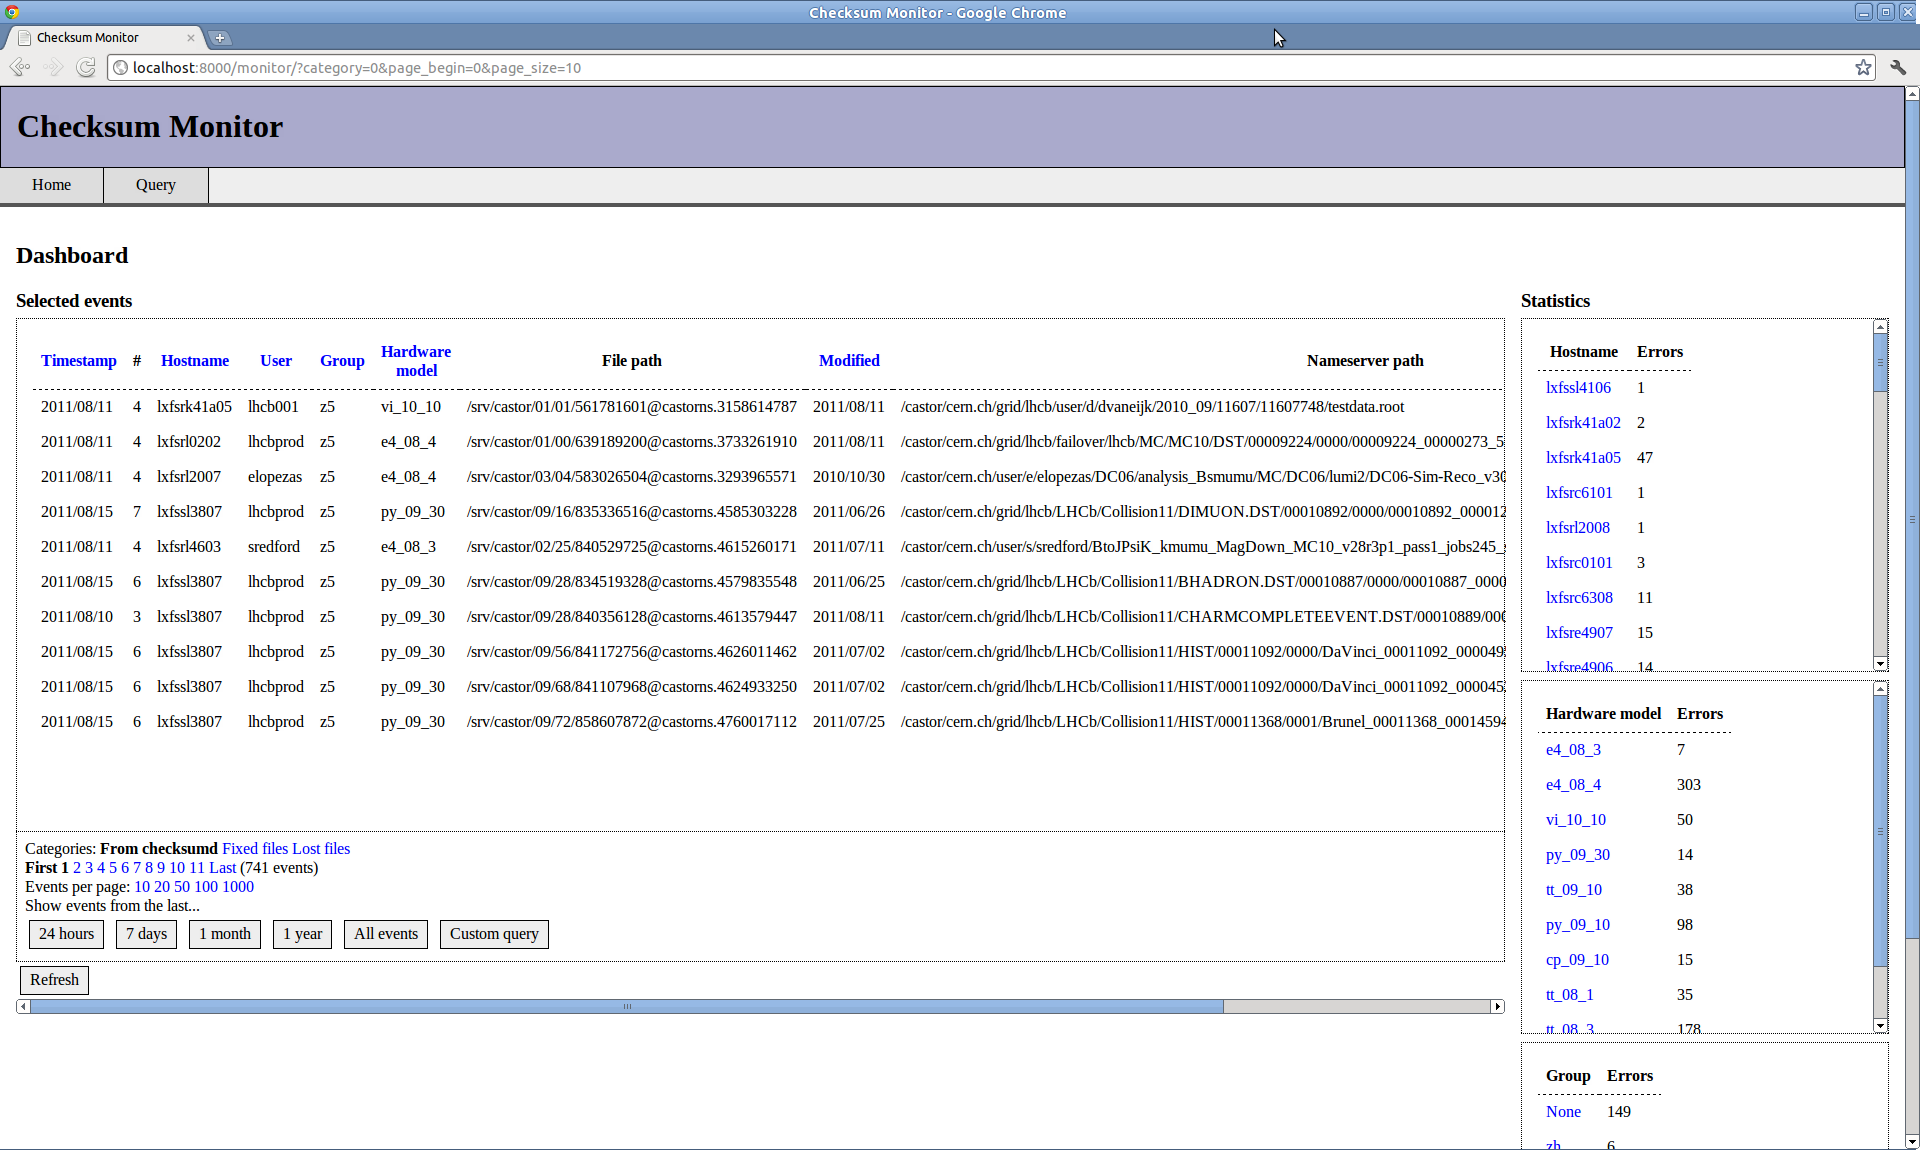
\includegraphics[width=\textwidth]{gfx/checksum-monitor-main}
\caption{Checksum monitor main page}
\label{fig:monitor-index}
\end{figure}

In addition to the main page, there is a search page which can be reached either by clicking "Query" in the menu or "Custom query" near the timespan buttons. The search form is shown in figure \ref{fig:monitor-search}. All the fields that are searched on are AND-ed, forming the final query. So specifying e.g. hostname "lxfsj4107" and category "fixed" searches for all events from host lxfsj4107 that are in the fixed category.

\begin{figure}[ht]
\centering
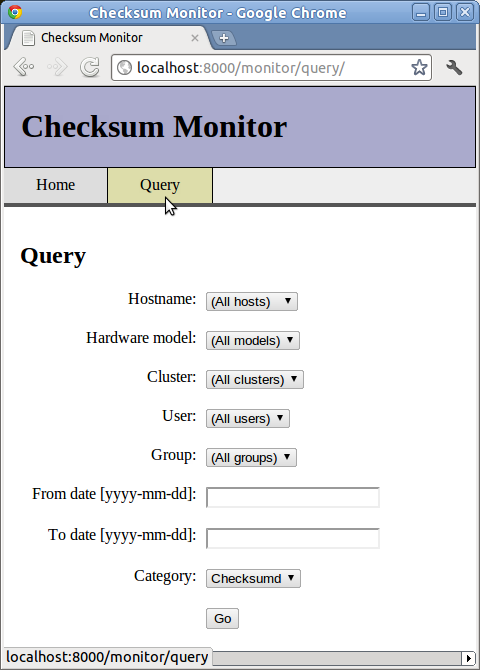
\includegraphics[width=0.5\textwidth]{gfx/checksum-monitor-search}
\caption{Checksum monitor search page}
\label{fig:monitor-search}
\end{figure}

